% !TeX program = xelatex
\documentclass[UTF8,11pt,a4paper,fontset=fandol]{ctexart}

\usepackage[a4paper,margin=2.35cm,headheight=15pt]{geometry}
\usepackage{amsmath,amssymb,bm}
\usepackage{graphicx}
\usepackage{booktabs,multirow,tabularx,longtable,array}
\usepackage{threeparttable}
\usepackage{float}
\usepackage{subcaption}
\usepackage{xcolor}
\usepackage{siunitx}
\usepackage{enumitem}
\usepackage{fancyhdr}
\usepackage{hyperref}
\usepackage{cleveref}
\usepackage{listings}
\usepackage{microtype}
\usepackage{seqsplit}

% Make Chinese paths render correctly in listings and \path commands.
\setCJKmonofont{FandolFang-Regular.otf}

\definecolor{linkblue}{RGB}{28,89,145}
\definecolor{codebg}{RGB}{247,248,250}
\hypersetup{
  colorlinks=true,
  linkcolor=linkblue,
  citecolor=linkblue,
  urlcolor=linkblue,
  pdftitle={单细胞药物扰动响应预测与剂量建模考核报告},
  pdfauthor={考生}
}
\graphicspath{{figures/}}
\setlength{\parindent}{2em}
\setlength{\parskip}{0.18em}
\setlist{nosep,leftmargin=2.2em}
\renewcommand{\arraystretch}{1.18}
\sisetup{round-mode=places,round-precision=4,detect-all}

\pagestyle{fancy}
\fancyhf{}
\fancyhead[L]{单细胞药物扰动响应预测与剂量建模}
\fancyhead[R]{考核报告}
\fancyfoot[C]{\thepage}

\lstset{
  basicstyle=\ttfamily\small,
  backgroundcolor=\color{codebg},
  frame=single,
  rulecolor=\color{black!15},
  breaklines=true,
  columns=fullflexible,
  keepspaces=true,
  showstringspaces=false
}

\newcommand{\scvidr}{\textsc{scVIDR}}
\newcommand{\dsdr}{\textsc{DSDR}}
\newcommand{\Rtwo}{\ensuremath{R^2}}

\title{\bfseries 南开大学推免生动手能力测试\\[0.8em]
\LARGE 单细胞药物扰动响应预测与剂量建模}
\author{考生：\underline{陈培杰}}
\date{2026年9月}

\begin{document}

\maketitle
\thispagestyle{empty}
\vspace{1.5cm}

\begin{abstract}
本报告基于 sci-Plex 3 单细胞化学扰动数据，完成了对未见细胞系--药物--剂量组合的表达预测，并研究了剂量响应函数的改进。实验以 A549 为目标细胞系，以 $(+)$-JQ1 和 Trametinib（GSK1120212）为目标药物；A549 的全部非零剂量样本仅用于测试，训练集只包含 A549 对照细胞及 K562、MCF7 的对照和给药细胞。首先训练 32 维变分自编码器，并通过潜空间扰动向量与跨细胞系线性回归构建条件特异的 \scvidr 预测。在 8 个测试条件上，全基因平均表达的 Pearson 相关系数为 0.9013--0.9885，\Rtwo 为 0.8096--0.9698，相比直接使用对照均值的基线在 5/8 条件上提高了 \Rtwo。

任务二保留上述原模型与代码，复现原始对数线性剂量缩放，并提出归一化 Hill 函数。Hill 模型在 6 个非最大剂量条件的 Top-100 差异表达基因上均取得 \Rtwo 提升，但全基因平均提升为负，说明单一标量缩放难以同时恢复所有剂量的响应方向。进一步提出剂量特异方向回归（dose-specific direction regression, \dsdr）：对每个药物--剂量直接估计独立潜空间响应并跨细胞系回归。\dsdr 在 6/6 个非最大剂量条件上提高 Top-100 DE \Rtwo，8 个条件平均增益为 0.0107，最大增益为 0.0348；其代价是全基因平均 \Rtwo 下降 0.0038。结果表明，剂量变化不仅改变扰动幅度，也会改变潜空间方向；在本数据划分下，\dsdr 对关键响应基因的恢复优于对数线性和 Hill 标量插值。
\end{abstract}

\noindent\textbf{关键词：} 单细胞转录组；药物扰动；变分自编码器；剂量响应；scVIDR；Hill 函数

\clearpage
\tableofcontents
\clearpage

\section{研究背景与任务目标}

大规模单细胞化学转录组实验可以同时测量细胞类型、药物和剂量对表达状态的影响，但完整覆盖所有组合的实验成本很高。sci-Plex 通过组合索引在单细胞分辨率下实现了大规模化学扰动测量\cite{srivatsan2020}。在此基础上，\scvidr 使用变分自编码器（variational autoencoder, VAE）学习表达流形，并用潜空间向量运算与回归预测未测细胞类型和未测剂量的响应\cite{kana2023}。

本次考核包含两个递进目标：

\begin{enumerate}
  \item 在严格留出 A549 给药样本的前提下，使用 K562、MCF7 的响应与 A549 对照细胞预测 A549 在两种药物、四个非零剂量下的表达；
  \item 复现原始对数线性剂量模型，设计更合理的剂量建模方法并比较其在全基因、高变基因及差异表达基因上的表现。
\end{enumerate}

所有模型选择和拟合均不使用 A549 给药测试表达。测试真值仅用于最终评价、绘图，以及在方法开发完成后的误差分析。

\section{数据与实验设计}

\subsection{数据来源与条件选择}

原始数据为 \texttt{SrivatsanTrapnell2020\_sciplex3.h5ad}，包含 799,317 个细胞和 110,983 个原始特征。实验固定 24 h 时间点，选择 A549 为目标细胞系，K562 和 MCF7 为源细胞系，选择 $(+)$-JQ1 与 Trametinib（GSK1120212）两种药物。每种药物均包含 10、100、1,000、10,000 nM 四个非零剂量及对照。

为控制计算量并保持条件平衡，对每个训练给药组最多随机抽取 300 个细胞，对每个细胞系的对照组最多抽取 500 个细胞。随机种子固定为 20260913。最终获得 6,892 个细胞，其中训练集 5,370 个、测试集 1,522 个。

\begin{table}[H]
\centering
\caption{训练集与测试集构成。A549 的全部非零剂量样本均被严格留出。}
\label{tab:split}
\begin{tabular}{llrrr}
\toprule
集合 & 细胞系与条件 & $(+)$-JQ1 & Trametinib & 合计 \\
\midrule
训练 & A549/K562/MCF7 对照 & \multicolumn{2}{c}{1,500} & 1,500 \\
训练 & K562 非零剂量 & 736 & 734 & 1,470 \\
训练 & MCF7 非零剂量 & 1,200 & 1,200 & 2,400 \\
\midrule
测试 & A549，10 nM & 174 & 167 & 341 \\
测试 & A549，100 nM & 183 & 176 & 359 \\
测试 & A549，1,000 nM & 218 & 210 & 428 \\
测试 & A549，10,000 nM & 223 & 171 & 394 \\
\midrule
\multicolumn{2}{r}{合计} & 2,934 & 2,858 & 6,892 \\
\bottomrule
\end{tabular}
\end{table}

\subsection{预处理与防止数据泄漏}

预处理参数仅在训练集上估计：首先保留在至少 20 个训练细胞中表达的基因；随后对每个细胞进行总量归一化至 $10^4$，再作 $\log(1+x)$ 变换；最后使用 Seurat dispersion 方法从训练集选择 2,000 个高变基因（HVG）。测试集只应用由训练集确定的基因集合与相同变换，不参与 HVG 选择、VAE 训练、潜空间回归或剂量函数拟合。

\subsection{评价指标}

对每个药物--剂量条件，先分别计算真实细胞与预测细胞的逐基因平均表达 $\bm{\mu}$，然后报告：

\begin{align}
r &= \operatorname{corr}(\bm{\mu}_{\mathrm{true}},\bm{\mu}_{\mathrm{pred}}), \\
R^2 &= 1-\frac{\sum_g(\mu_{g,\mathrm{true}}-\mu_{g,\mathrm{pred}})^2}
{\sum_g(\mu_{g,\mathrm{true}}-\bar{\mu}_{\mathrm{true}})^2}.
\end{align}

指标分别在全部 2,000 个保留基因、Top-500 HVG 和 Top-100 DE 基因上计算。每个测试条件的 Top-100 DE 基因由该条件真实给药细胞与 A549 对照细胞的平均表达差绝对值排序得到，因此它是\emph{评价集合}，不参与训练。UMAP 则将对照、真实与各方法预测细胞放入共同的 log-normalized 表达矩阵中，联合执行 PCA、邻居图和 UMAP，避免不同嵌入坐标系造成视觉误判。

\section{方法}

\subsection{VAE 表达流形}

编码器以表达向量 $\bm{x}$ 为输入，输出近似后验 $q_{\phi}(\bm{z}\mid\bm{x})$ 的均值和方差；通过重参数化采样低维变量 $\bm{z}$，解码器 $p_{\theta}(\bm{x}\mid\bm{z})$ 重构表达。训练目标为重构损失与 KL 散度之和：

\begin{equation}
\mathcal{L}(\theta,\phi)=
\mathbb{E}_{q_{\phi}(\bm{z}\mid\bm{x})}
\left[\lVert\bm{x}-\hat{\bm{x}}\rVert_2^2\right]
+\beta D_{\mathrm{KL}}\!\left(q_{\phi}(\bm{z}\mid\bm{x})\,\|\,\mathcal{N}(\bm{0},\bm{I})\right).
\end{equation}

本实验的编码器和解码器均使用两层 256 单元全连接网络，潜变量维度为 32，dropout 为 0.15，最多训练 60 个 epoch，早停 patience 为 15。

\subsection{任务一：条件特异的 scVIDR 预测}

对源细胞系 $c\in\{\mathrm{K562},\mathrm{MCF7}\}$、药物 $p$ 和剂量 $d$，计算潜空间中心差：

\begin{equation}
\Delta_{c,p,d}=\bar{\bm{z}}_{c,p,d}-\bar{\bm{z}}_{c,\mathrm{control}}.
\end{equation}

对每个条件 $(p,d)$，在源细胞系上拟合从对照中心到响应向量的逐维线性关系，并在 A549 对照中心处外推得到 $\widehat{\Delta}_{\mathrm{A549},p,d}$。将其加到每个 A549 对照细胞的潜表示，再经解码器得到预测：

\begin{equation}
\hat{\bm{x}}_{i,p,d}=D_{\theta}\!\left(E_{\phi}(\bm{x}_{i,\mathrm{A549,ctrl}})
+\widehat{\Delta}_{\mathrm{A549},p,d}\right).
\end{equation}

该实现对每个观测剂量独立建模，是任务一的正式结果，也为后续 \dsdr 方法提供了方向。

\subsection{任务二原模型：对数线性缩放}

原始多剂量模型只用最大剂量估计目标细胞系的潜空间扰动方向 $\widehat{\Delta}_{p,d_{\max}}$，中间剂量按对数剂量比例缩放：

\begin{equation}
\alpha_{\log}(d)=\frac{\log(d+1)}{\log(d_{\max}+1)},\qquad
\widehat{\Delta}_{p,d}=\alpha_{\log}(d)\widehat{\Delta}_{p,d_{\max}}.
\label{eq:log}
\end{equation}

这种参数化稳定且无需额外拟合，但隐含两个强假设：所有剂量共享同一潜空间方向；响应幅度严格服从固定的对数比例。

\subsection{改进一：归一化 Hill 剂量函数}

为允许低剂量阈值、转折区和高剂量饱和，使用归一化 Hill 函数替代式\eqref{eq:log}：

\begin{equation}
\alpha_{\mathrm{Hill}}(d)=
\frac{d^h/(EC_{50}^h+d^h)}
{d_{\max}^h/(EC_{50}^h+d_{\max}^h)}.
\end{equation}

其中 $h$ 为 Hill 系数，$EC_{50}$ 控制曲线转折位置。先在 K562 和 MCF7 上将各剂量响应向量投影到最大剂量方向，得到训练响应比例，再以 soft-$L_1$ 鲁棒损失按药物拟合 $h$ 与 $EC_{50}$。整个拟合过程不使用 A549 给药数据。

\subsection{改进二：剂量特异方向回归（DSDR）}

Hill 函数仍然只能改变最大剂量方向的长度，无法描述剂量导致的响应方向旋转。为此进一步提出 \dsdr。对每个 $(p,d)$，直接使用 K562 和 MCF7 的完整潜空间响应向量 $\Delta_{c,p,d}$，逐潜变量维度回归到 A549 对照中心：

\begin{align}
\Delta_{c,p,d,j} &= a_{p,d,j}\,\bar z_{c,\mathrm{ctrl},j}+b_{p,d,j},\\
\widehat{\Delta}_{\mathrm{A549},p,d,j}
&=a_{p,d,j}\,\bar z_{\mathrm{A549,ctrl},j}+b_{p,d,j}.
\end{align}

与对数线性和 Hill 模型相比，\dsdr 不再要求
$\widehat{\Delta}_{p,d}\parallel\widehat{\Delta}_{p,d_{\max}}$，允许每个剂量拥有独立的响应方向。它不增加 VAE 训练次数，代价是每个待预测剂量必须在至少两个源细胞系中有观测。

\section{任务一结果：A549 未见扰动预测}

\subsection{定量结果}

\cref{tab:task1} 给出了条件特异 \scvidr 在全部 2,000 个基因上的结果。Pearson 系数均高于 0.90，\Rtwo 均高于 0.80。$(+)$-JQ1 在低剂量下最易预测，10 nM 时达到 $r=0.9885$、$R^2=0.9698$；随剂量升高，预测难度增加。Trametinib 的整体相关性相对较低，但各剂量仍保持 $R^2\geq0.8096$。

\begin{table}[H]
\centering
\begin{threeparttable}
\caption{任务一：A549 各测试条件的全基因平均表达预测。}
\label{tab:task1}
\begin{tabular}{lrrrr}
\toprule
药物 & 剂量/nM & Pearson $r$ & scVIDR $R^2$ & 对照基线 $R^2$ \\
\midrule
\multirow{4}{*}{$(+)$-JQ1}
 & 10 & 0.9885 & 0.9698 & 0.9820 \\
 & 100 & 0.9759 & 0.9486 & 0.9461 \\
 & 1,000 & 0.9454 & 0.8930 & 0.8486 \\
 & 10,000 & 0.9372 & 0.8738 & 0.8200 \\
\midrule
\multirow{4}{*}{Trametinib}
 & 10 & 0.9141 & 0.8295 & 0.8380 \\
 & 100 & 0.9175 & 0.8415 & 0.8253 \\
 & 1,000 & 0.9048 & 0.8096 & 0.8147 \\
 & 10,000 & 0.9013 & 0.8111 & 0.7872 \\
\bottomrule
\end{tabular}
\begin{tablenotes}[flushleft]\small
\item 对照基线指直接以 A549 对照平均表达预测给药后的平均表达。scVIDR 在 5/8 个条件上获得更高的 $R^2$。
\end{tablenotes}
\end{threeparttable}
\end{table}

Top-100 DE 基因上的 $R^2$ 对 $(+)$-JQ1 分别为 0.9250、0.9112、0.8156、0.7480，对 Trametinib 分别为 0.5543、0.6544、0.4605、0.4610。与全基因结果相比，DE 基因上的性能明显降低，说明高动态响应基因是模型的主要误差来源，单看全基因相关性会因大量稳定基因而高估扰动恢复能力。

\begin{figure}[H]
\centering
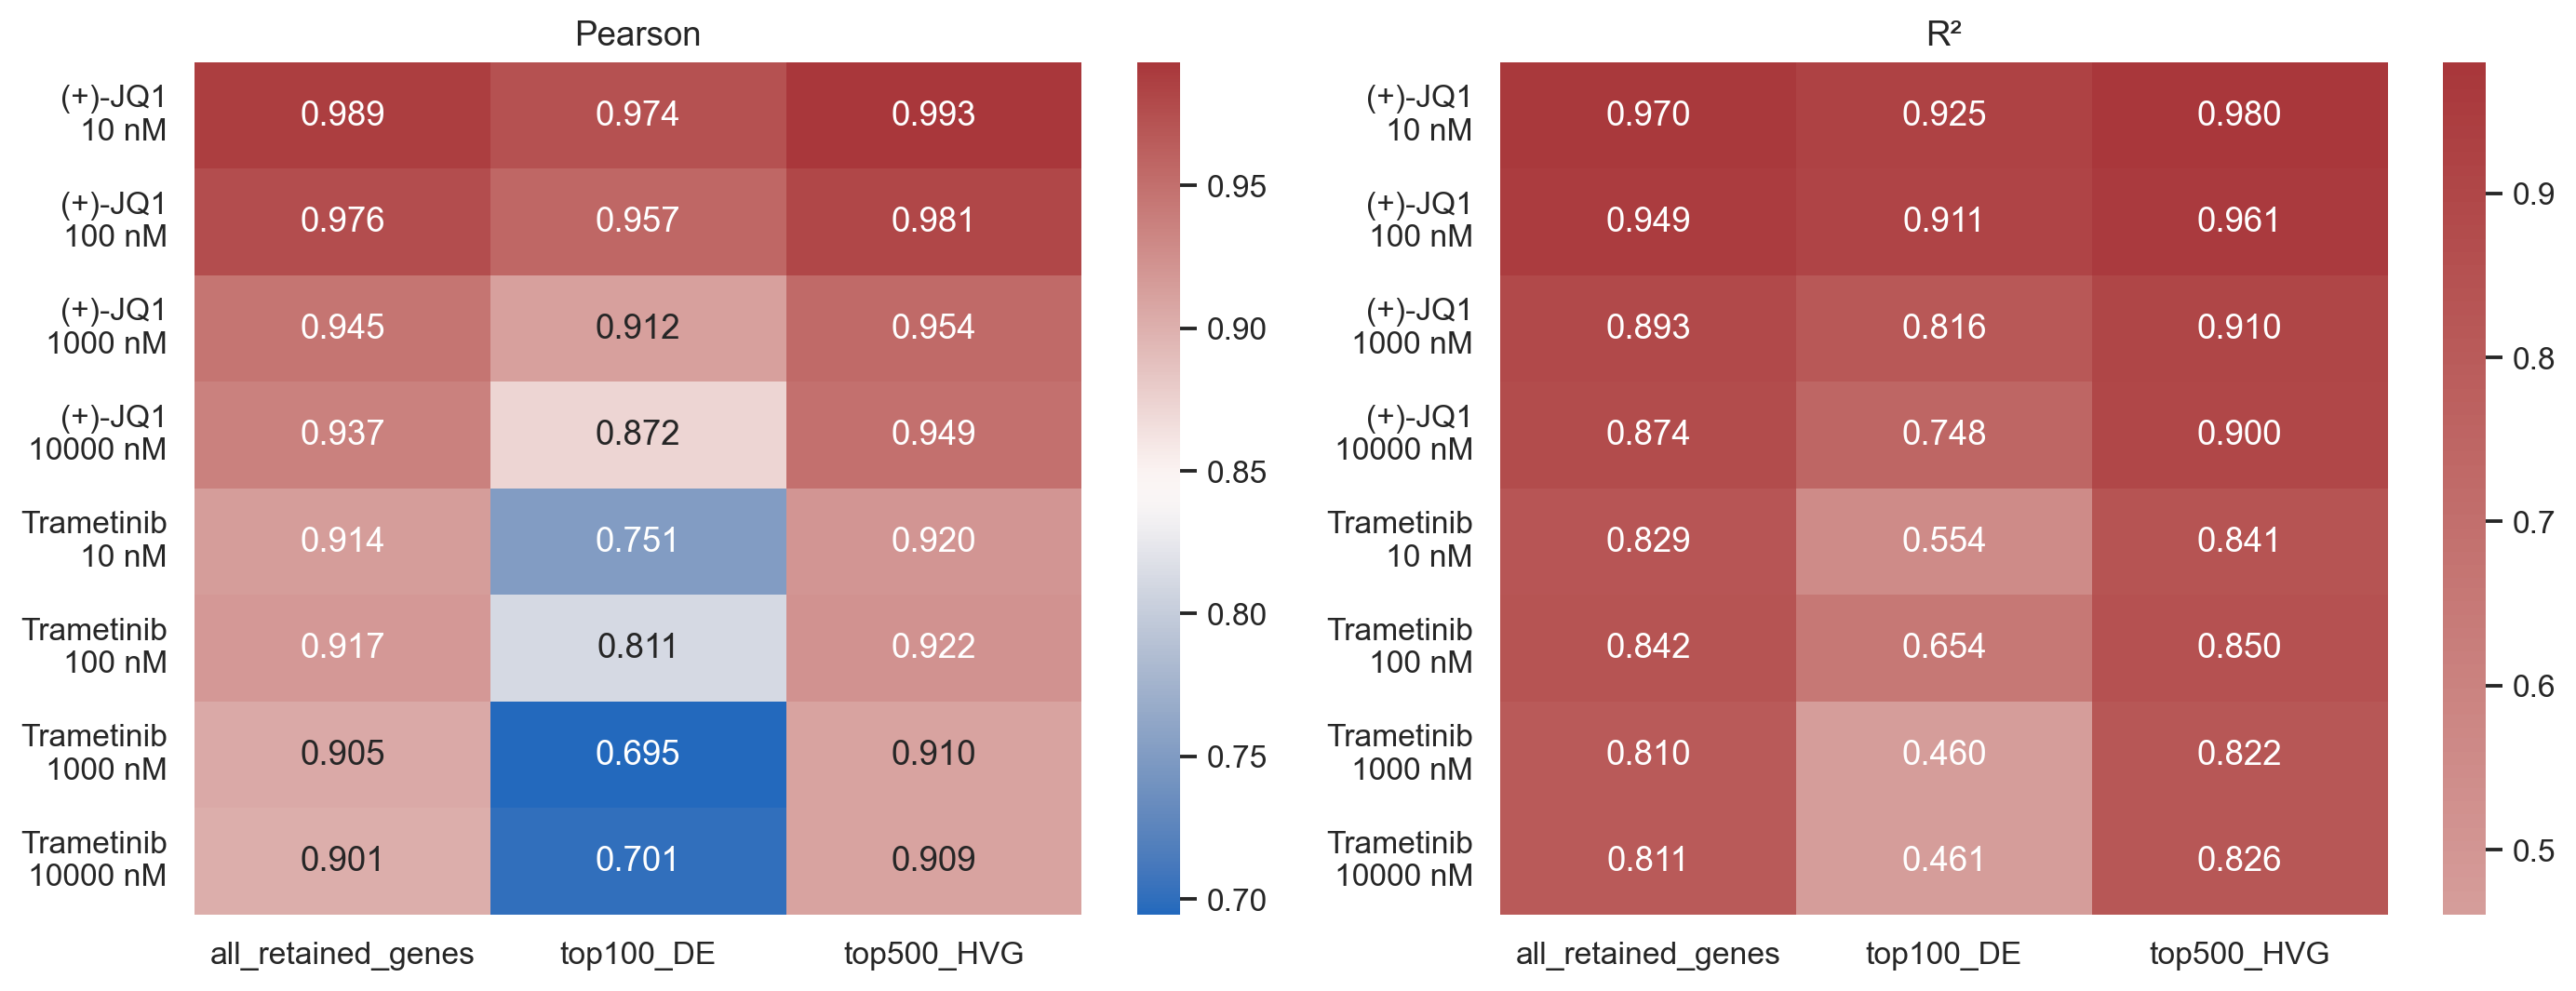
\includegraphics[width=0.98\textwidth]{task1_metric_heatmaps.png}
\caption{任务一各药物、剂量和基因集合上的 Pearson 与 $R^2$。}
\label{fig:task1metrics}
\end{figure}

\subsection{共同 UMAP 分布}

\cref{fig:task1umap} 显示预测细胞总体位于 A549 表达流形附近，并能随药物和剂量发生位移；但预测分布通常比真实分布更集中，局部形状并未完全重合。这与 VAE 重构及中心向量平移的机制一致：模型更擅长恢复条件平均状态，而不保证细胞间异质性和高阶分布统计量完全正确。

\begin{figure}[H]
\centering
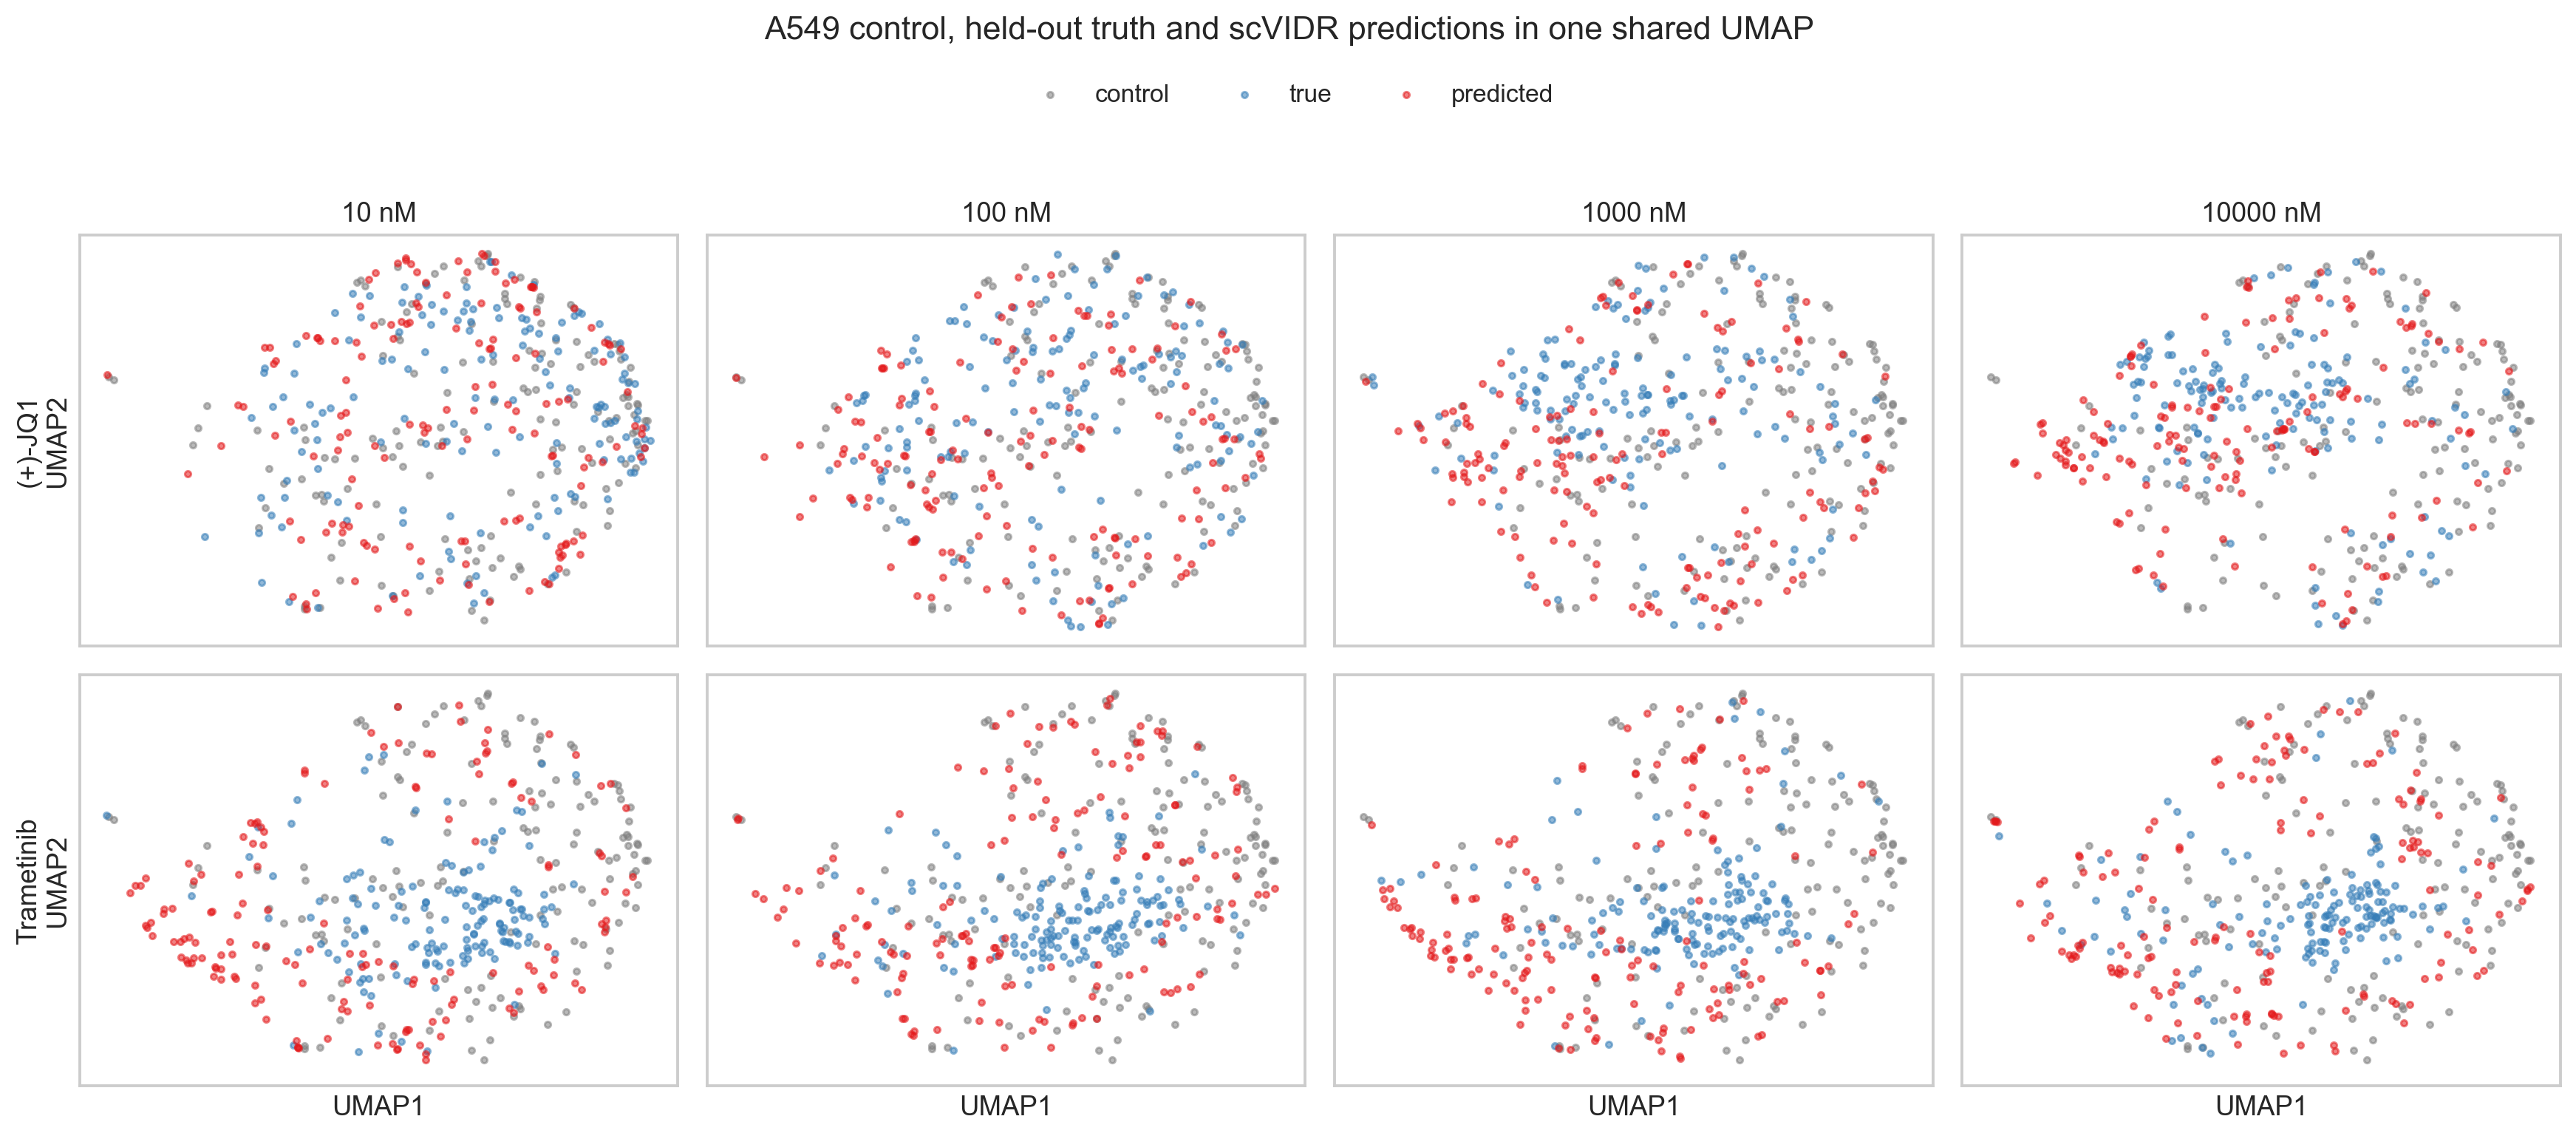
\includegraphics[width=0.98\textwidth]{task1_umap.png}
\caption{A549 对照、真实给药细胞与任务一预测细胞的共同 UMAP。}
\label{fig:task1umap}
\end{figure}

\section{任务二结果：剂量函数改进}

\subsection{Hill 模型拟合}

源细胞系数据拟合得到 $(+)$-JQ1 的 $h=0.8145$、$EC_{50}=70.75$ nM，训练投影比例 RMSE 为 0.0634。Trametinib 的拟合结果为 $h=0.1$、$EC_{50}=0.001$ nM，二者均触及设定下界，RMSE 为 0.1030。后者应解释为“在现有四个非零剂量上响应较早饱和，最优数值形状接近平台”，不能把该 $EC_{50}$ 当作可靠的生理药效参数。

\begin{figure}[H]
\centering
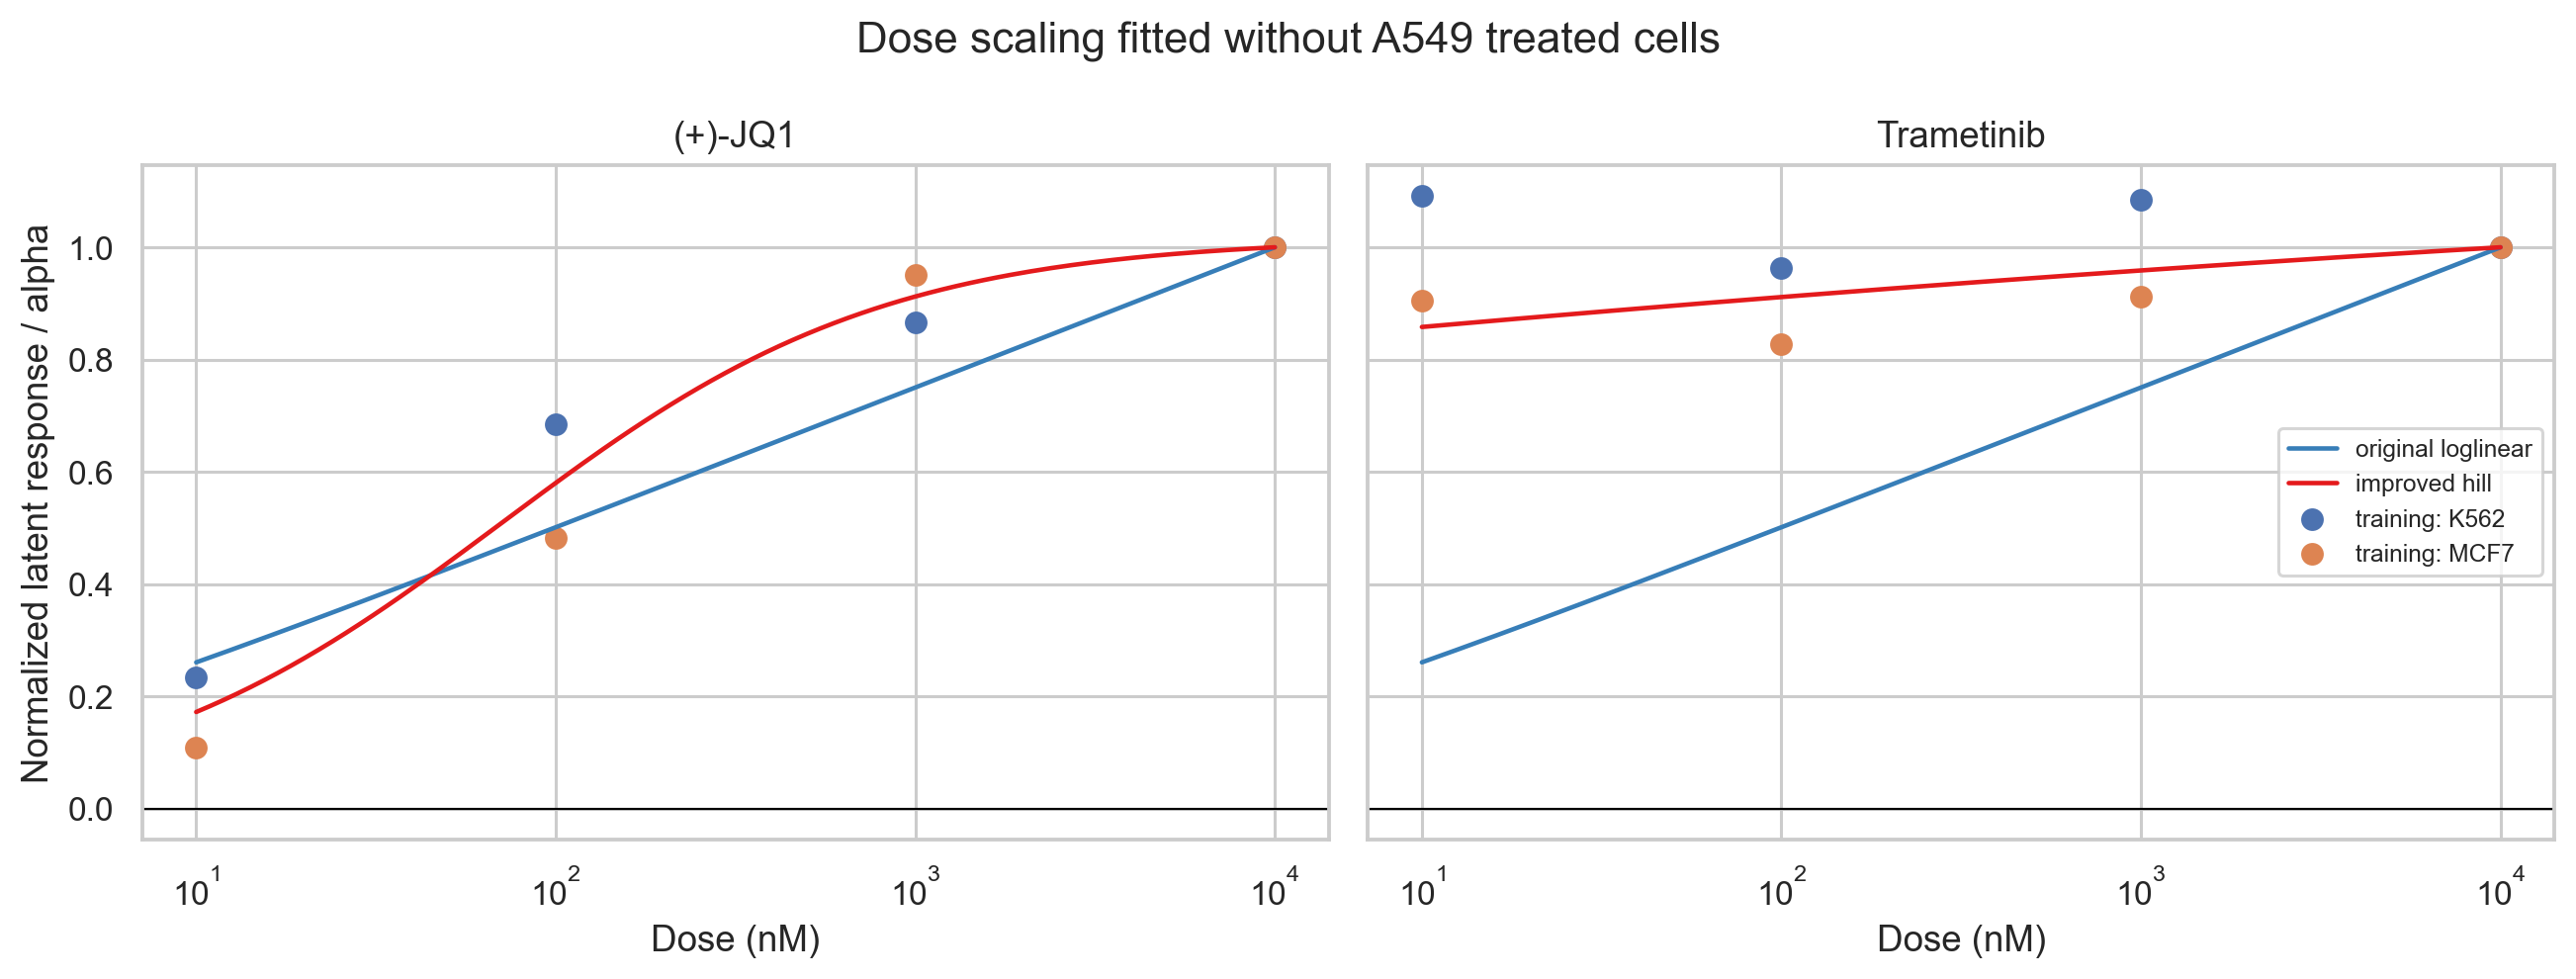
\includegraphics[width=0.92\textwidth]{dose_scaling.png}
\caption{原始对数线性缩放、拟合 Hill 缩放与源细胞系观测响应比例。}
\label{fig:scaling}
\end{figure}

\subsection{原模型与 Hill 模型比较}

Hill 模型在 6 个非最大剂量条件的 Top-100 DE 基因上全部提高 $R^2$，8 个条件的平均增益为 0.0075；其中 Trametinib 10 nM 的增益最大，为 0.0172。最大剂量被归一化为 1，因此两种模型在 10,000 nM 上完全相同。

然而，Hill 在全部基因上的平均 $R^2$ 增益为 $-0.0021$，仅在 1/8 条件上超过原始模型；Top-100 DE 的 Pearson 平均增益也约为 $-0.0006$。这说明 Hill 曲线更接近关键响应基因的剂量幅度，但一个药物共享的标量函数仍不能同时解释不同基因模块和不同潜变量方向。

\begin{table}[H]
\centering
\caption{Top-100 DE 基因上的原始对数线性与 Hill 模型 $R^2$。}
\label{tab:hill}
\begin{tabular}{lrrrr}
\toprule
药物 & 剂量/nM & 对数线性 & Hill & Hill 增益 \\
\midrule
\multirow{4}{*}{$(+)$-JQ1}
 & 10 & 0.9157 & 0.9217 & +0.0061 \\
 & 100 & 0.9086 & 0.9089 & +0.0003 \\
 & 1,000 & 0.8027 & 0.8147 & +0.0121 \\
 & 10,000 & 0.7377 & 0.7377 & 0.0000 \\
\midrule
\multirow{4}{*}{Trametinib}
 & 10 & 0.5441 & 0.5614 & +0.0172 \\
 & 100 & 0.6416 & 0.6544 & +0.0128 \\
 & 1,000 & 0.4320 & 0.4433 & +0.0113 \\
 & 10,000 & 0.4659 & 0.4659 & 0.0000 \\
\bottomrule
\end{tabular}
\end{table}

\begin{figure}[H]
\centering
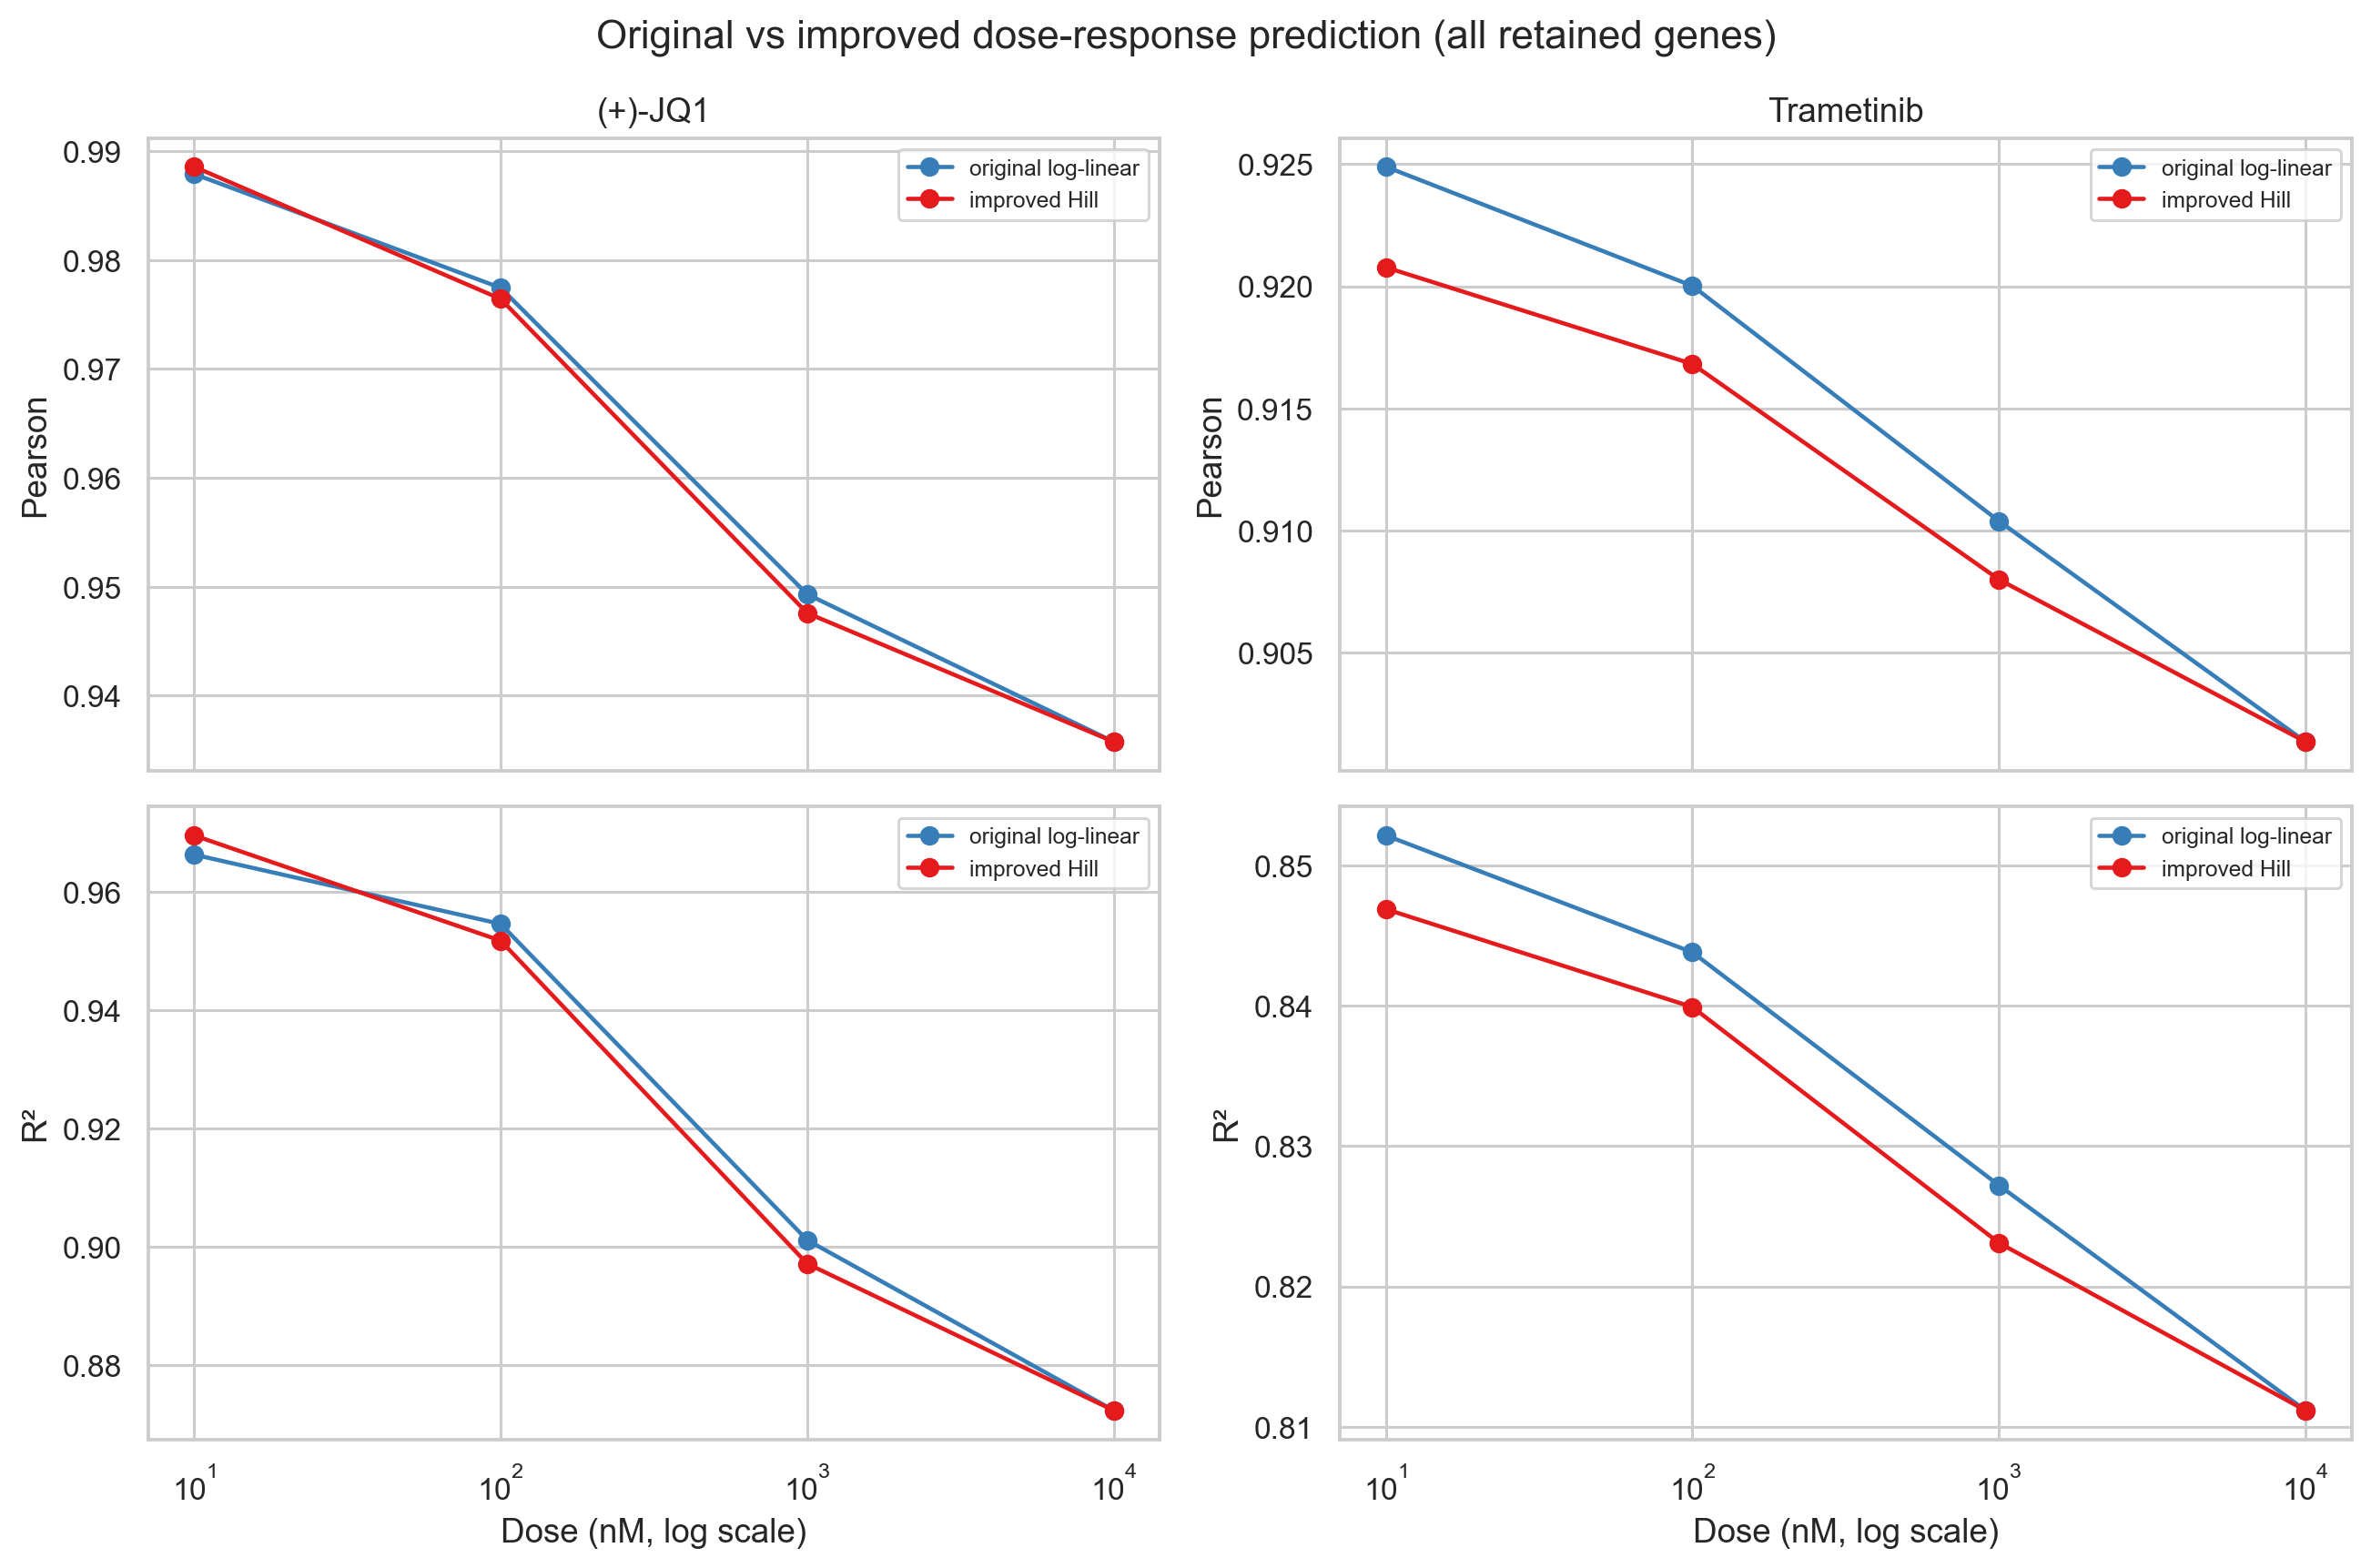
\includegraphics[width=0.98\textwidth]{hill_metrics.png}
\caption{对数线性与 Hill 模型的逐剂量指标比较。}
\label{fig:hillmetrics}
\end{figure}

\section{进一步改进：剂量特异方向回归}

\subsection{核心结果}

\dsdr 在 6/6 个非最大剂量条件上提高 Top-100 DE 的 $R^2$；8 个条件（包含两个固定不变的最大剂量）的平均增益为 0.0107，高于 Hill 的 0.0075。最大提升出现在 Trametinib 1,000 nM，$R^2$ 从 0.4320 增至 0.4668，增益为 0.0348。Trametinib 100 nM 也由 0.6416 提升至 0.6610。

\begin{table}[H]
\centering
\caption{Top-100 DE 基因上三种剂量方法的 $R^2$。粗体为非最大剂量下的最优值。}
\label{tab:three}
\begin{tabular}{lrrrrr}
\toprule
药物 & 剂量/nM & 对数线性 & Hill & DSDR & DSDR 对原模型增益 \\
\midrule
\multirow{4}{*}{$(+)$-JQ1}
 & 10 & 0.9157 & \textbf{0.9217} & 0.9161 & +0.0004 \\
 & 100 & 0.9086 & 0.9089 & \textbf{0.9118} & +0.0032 \\
 & 1,000 & 0.8027 & \textbf{0.8147} & 0.8136 & +0.0110 \\
 & 10,000 & 0.7377 & 0.7377 & 0.7377 & 0.0000 \\
\midrule
\multirow{4}{*}{Trametinib}
 & 10 & 0.5441 & \textbf{0.5614} & 0.5611 & +0.0170 \\
 & 100 & 0.6416 & 0.6544 & \textbf{0.6610} & +0.0194 \\
 & 1,000 & 0.4320 & 0.4433 & \textbf{0.4668} & +0.0348 \\
 & 10,000 & 0.4659 & 0.4659 & 0.4659 & 0.0000 \\
\midrule
\multicolumn{2}{r}{8 条件平均增益} & --- & +0.0075 & \textbf{+0.0107} & \\
\bottomrule
\end{tabular}
\end{table}

\begin{figure}[H]
\centering
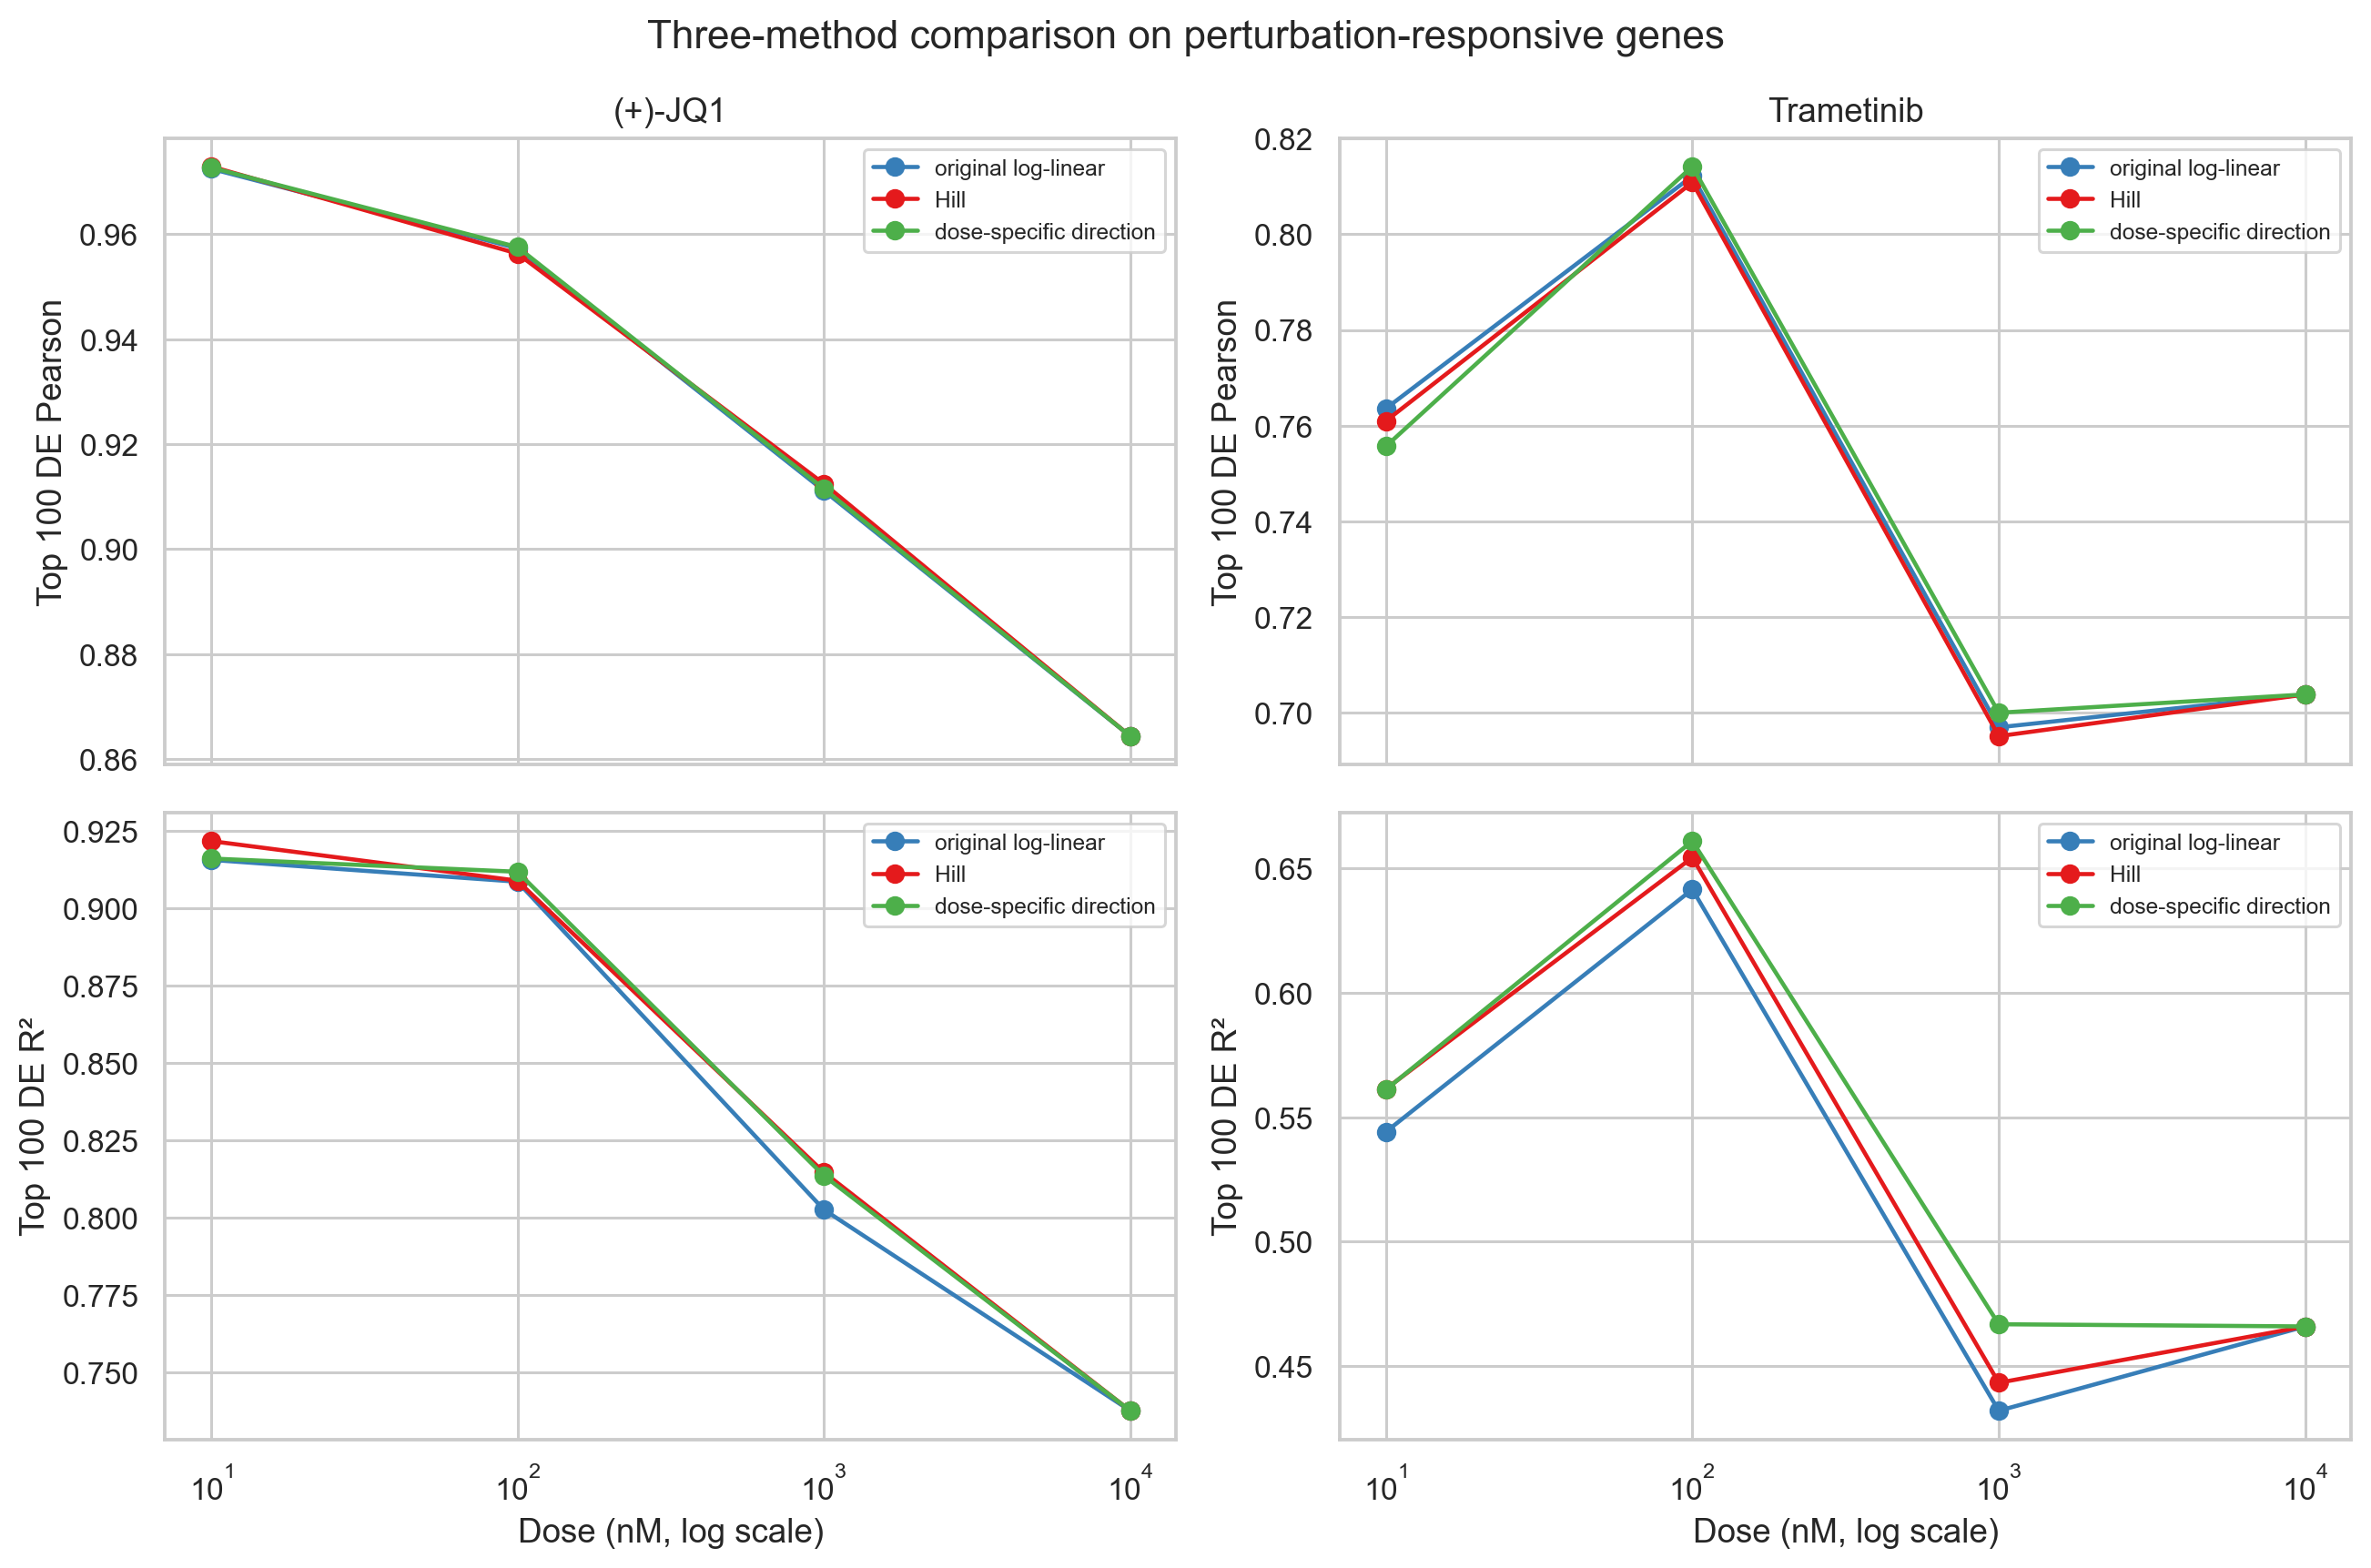
\includegraphics[width=0.98\textwidth]{dsdr_metrics.png}
\caption{对数线性、Hill 与 DSDR 的逐剂量指标及相对原模型的增益。}
\label{fig:dsdrmetrics}
\end{figure}

\subsection{代表性基因与分布可视化}

\cref{fig:genes} 展示了 $(+)$-JQ1 的 KRT81 和 Trametinib 的 ASPH。二者均从相应药物高剂量 Top-100 DE 基因中选择，并按 \dsdr 相对原模型的剂量曲线 RMSE 改善排序，仅用于事后解释而非训练。图中可见，\dsdr 的优势主要来自中间剂量位置的调整，而非简单地将整条曲线整体放大或缩小。

\begin{figure}[H]
\centering
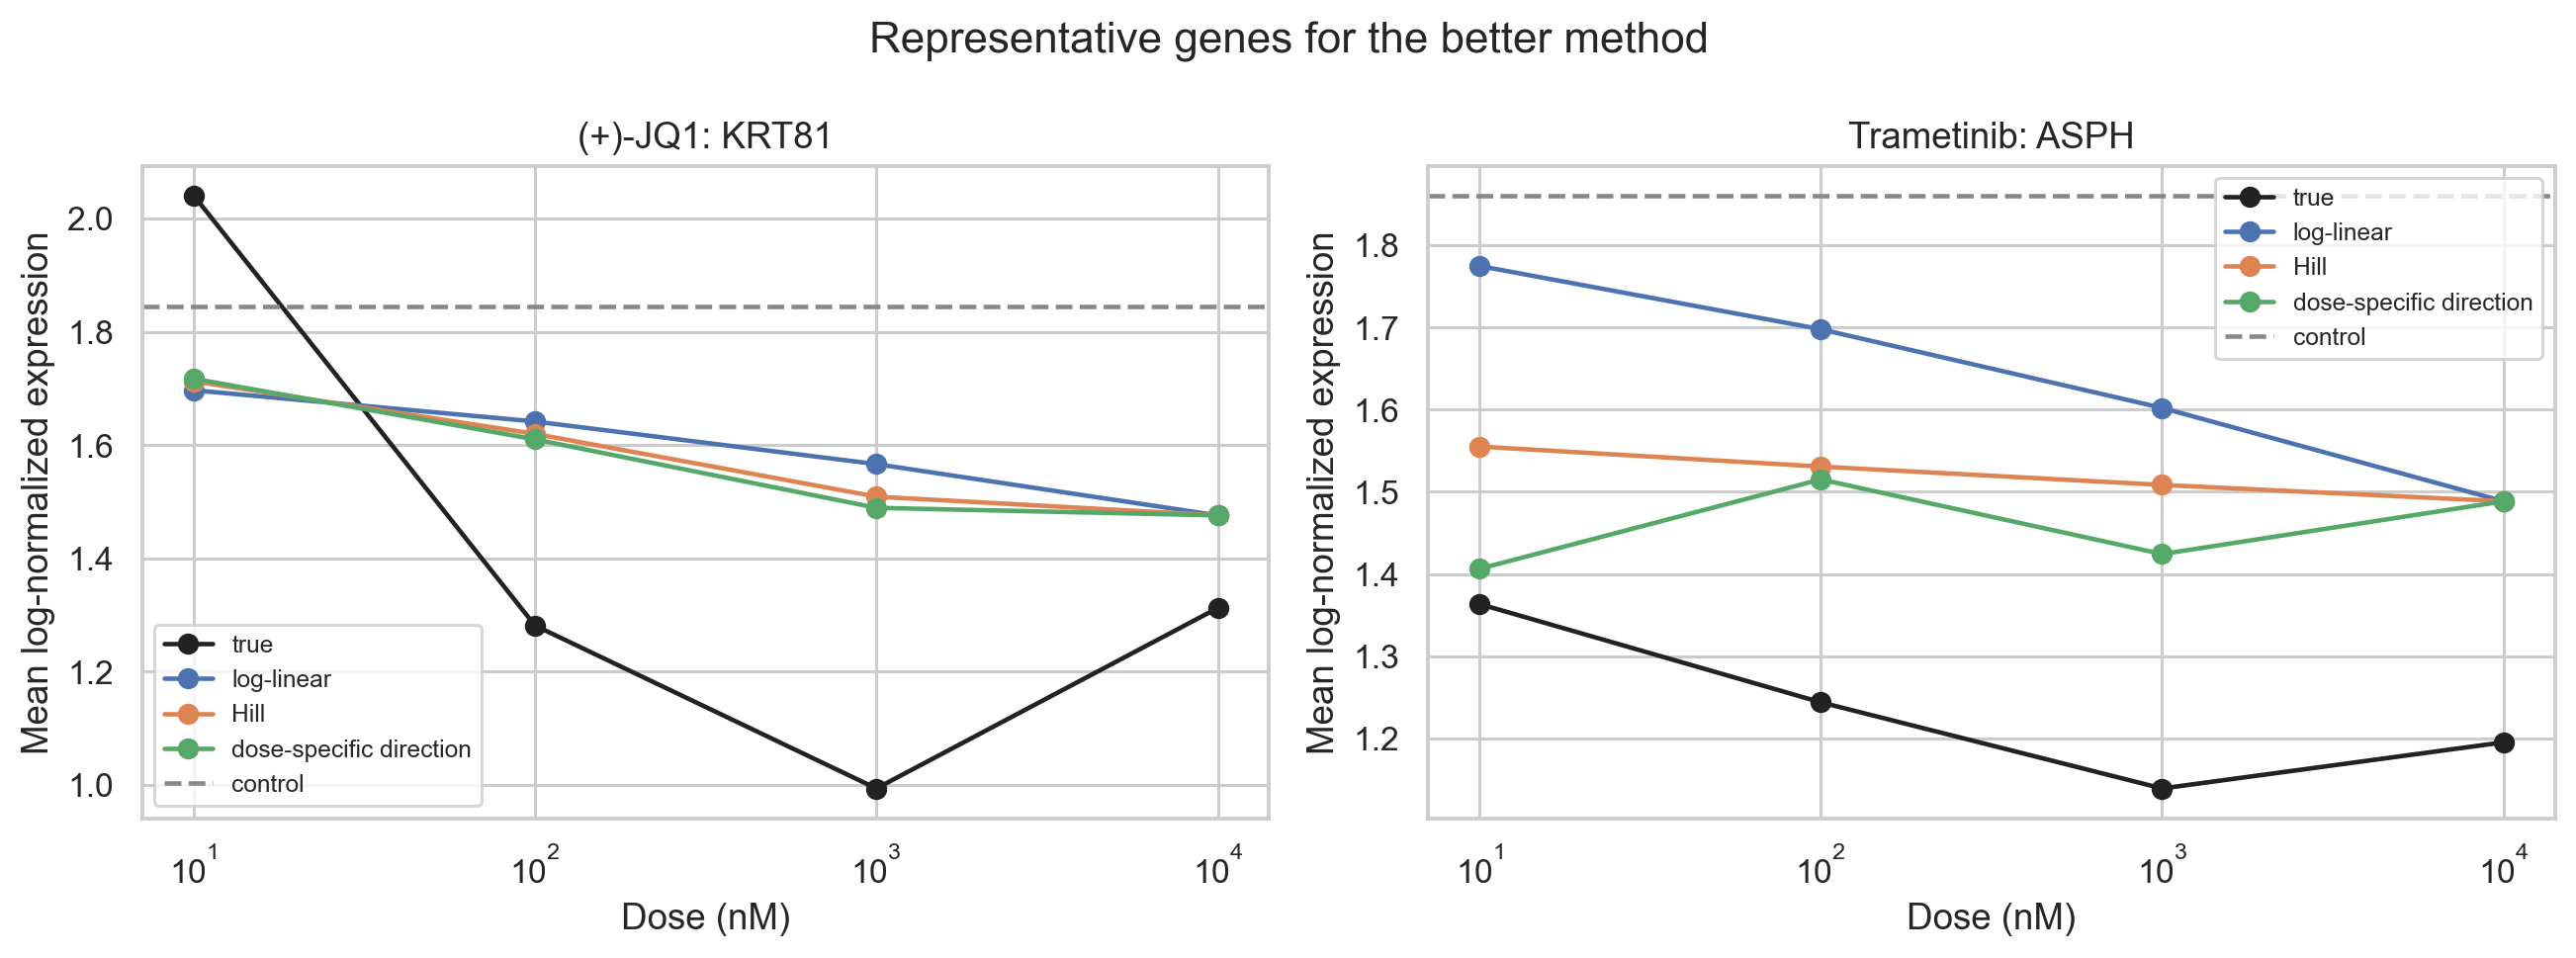
\includegraphics[width=0.92\textwidth]{dsdr_gene_curves.png}
\caption{代表性差异表达基因的真实与预测剂量曲线。}
\label{fig:genes}
\end{figure}

共同 UMAP 中三种模型的总体位置相近，说明平均表达指标上的改进并未造成明显的流形偏离；但预测分布仍比真实分布更集中，且不同方法间的局部差异较小。因此，UMAP 只作为分布结构的定性检查，主要结论仍以预先定义的逐条件定量指标为依据。

\begin{figure}[H]
\centering
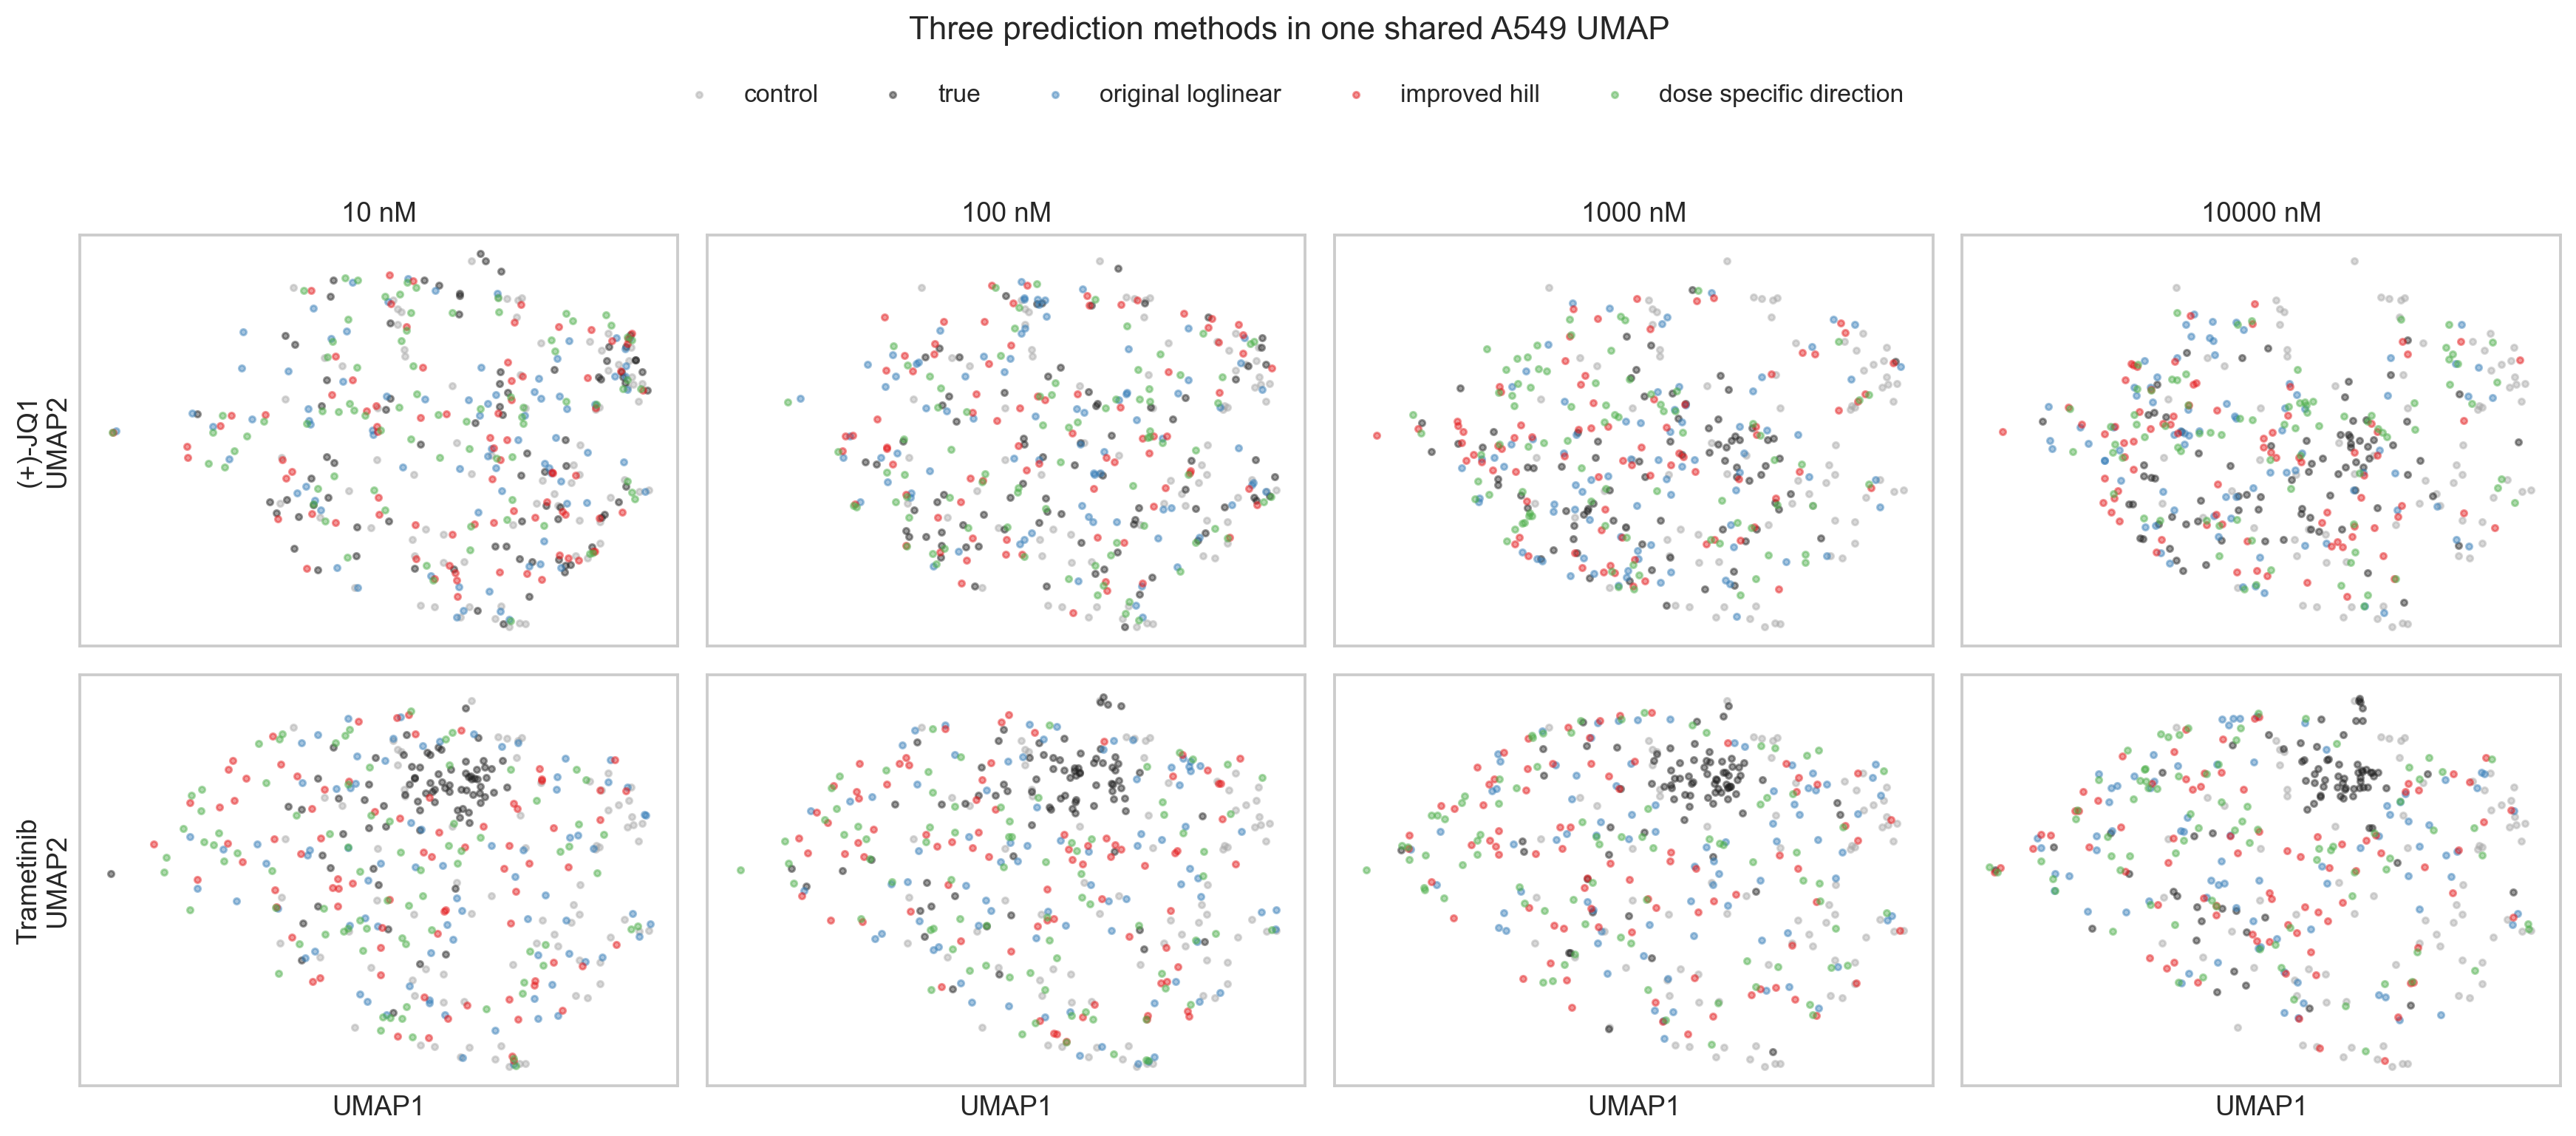
\includegraphics[width=0.98\textwidth]{dsdr_umap.png}
\caption{真实细胞、对照细胞及三种剂量模型预测的共同 UMAP。}
\label{fig:dsdrumap}
\end{figure}

\subsection{整体表达与关键响应之间的权衡}

\dsdr 的全基因平均 $R^2$ 相对对数线性模型下降 0.0038，Top-100 DE Pearson 平均增益约为 $-0.0003$。这并不与 Top-100 DE $R^2$ 的提升矛盾：Pearson 主要衡量跨基因排序和线性一致性，而 $R^2$ 对预测偏差与尺度误差敏感；全基因集合又由大量变化较小的基因主导。\dsdr 修正了响应最强基因在中间剂量的绝对表达偏差，却可能给大量稳定基因引入轻微偏移。因此，本方法的结论应准确表述为：\emph{更好地恢复关键差异表达响应，而非在所有评价口径上全面优于原模型}。

\section{探索性方法与误差分析}

在确定 \dsdr 前，还评估了若干训练数据驱动的替代方案。所有探索均保留为独立代码和结果文件，未覆盖正式原模型。

\begin{table}[H]
\centering
\caption{未选为最终方法的探索性方案及平均 $R^2$ 增益。}
\label{tab:negative}
\begin{tabularx}{\textwidth}{lrrX}
\toprule
方法 & 全基因 & Top-100 DE & 结论 \\
\midrule
校准的经验单调缩放 & $-0.0022$ & $+0.0082$ & 有效但弱于 DSDR，仍受单方向假设限制 \\
残差迁移 & $-0.0022$ & $-0.0026$ & 源细胞系残差不能稳定迁移至 A549 \\
DE 门控混合 & $-0.0016$ & $+0.0028$ & 提升较小，且引入基因级权重复杂度 \\
目标对照锚定 & $-0.0015$ & $-0.0328$ & 对关键响应基因造成明显退化 \\
\bottomrule
\end{tabularx}
\end{table}

这些负结果说明，仅增加曲线灵活性或对目标对照进行后处理，并不必然改善跨细胞系外推。真正有效的改动是放松“各剂量方向相同”这一结构假设。另一方面，\dsdr 目前仅有两个源细胞系，逐维线性回归的可辨识性有限；未来可加入更多源细胞系、岭回归或层次贝叶斯收缩，并通过留一源细胞系交叉验证选择模型复杂度。

\section{结论}

本次考核在无 A549 给药训练数据的严格设置下完成了两种药物、四个剂量的单细胞表达预测。任务一的条件特异 \scvidr 在全基因平均表达上取得 0.9013--0.9885 的 Pearson 和 0.8096--0.9698 的 $R^2$，证明潜空间扰动迁移能够较好地预测未见细胞系响应；与此同时，Top-100 DE 指标和共同 UMAP 揭示了强响应基因与细胞异质性仍是主要难点。

任务二完整保留并复现了原始对数线性模型。归一化 Hill 函数在所有非最大剂量的 Top-100 DE $R^2$ 上均优于原模型，验证了非线性饱和剂量曲线的价值。进一步提出的 \dsdr 允许潜空间响应方向随剂量变化，将平均 Top-100 DE $R^2$ 增益提高到 0.0107，并在 Trametinib 1,000 nM 达到 0.0348 的最大提升。综合结果支持如下判断：对于关键差异表达基因，剂量依赖不仅是扰动强度的变化，也包含响应方向的变化；若任务目标侧重机制相关的强响应基因，\dsdr 是本实验中更合适的方法；若目标是所有基因的整体平均拟合，则原始对数线性模型仍更稳健。

\section{可复现性与产物说明}

实验环境为 Windows、Python 3.8.5、Scanpy 1.9.1、AnnData 0.8.0、PyTorch 1.8.1+cu111，GPU 为 NVIDIA GeForce RTX 3070 Laptop。使用以下命令可分别复现任务一、任务二和进一步改进：

\begin{quote}\small
\texttt{conda activate scVIDR}\\
\texttt{python }任务一/\texttt{run\_task1.py}\\
\texttt{python }任务二/\texttt{run\_task2.py}\\
\texttt{python }任务二/\texttt{run\_better\_method.py}
\end{quote}

任务一完整模型、预测数据、指标及图表位于“任务一/”；任务二的原始模型、Hill 模型、\dsdr、探索性代码与全部结果位于“任务二/”。原任务一脚本的 SHA-256 为：
\begin{quote}\footnotesize
\texttt{\seqsplit{AE1F41910C431B8F94DF3ECED930DC0A36FA29D2520BF703BB34C7D8037C52FF}}
\end{quote}
该值同时记录于“任务二/\texttt{preservation\_manifest.json}”，用于证明原模型代码未被覆盖。本报告的源文件、PDF 和自包含图像位于“报告/”。

\begin{thebibliography}{9}
\bibitem{srivatsan2020}
Srivatsan SR, McFaline-Figueroa JL, Ramani V, et al.
Massively multiplex chemical transcriptomics at single-cell resolution.
\textit{Science}, 2020, 367(6473): 45--51.
doi: \href{https://doi.org/10.1126/science.aax6234}{10.1126/science.aax6234}.

\bibitem{kana2023}
Kana O, Nault R, Filipovic D, Marri D, Zacharewski T, Bhattacharya S.
Generative modeling of single-cell gene expression for dose-dependent chemical perturbations.
\textit{Patterns}, 2023, 4(8): 100817.
doi: \href{https://doi.org/10.1016/j.patter.2023.100817}{10.1016/j.patter.2023.100817}.

\bibitem{kingma2014}
Kingma DP, Welling M.
Auto-Encoding Variational Bayes.
\textit{International Conference on Learning Representations}, 2014.

\bibitem{lotfollahi2019}
Lotfollahi M, Wolf FA, Theis FJ.
scGen predicts single-cell perturbation responses.
\textit{Nature Methods}, 2019, 16: 715--721.
doi: \href{https://doi.org/10.1038/s41592-019-0494-8}{10.1038/s41592-019-0494-8}.
\end{thebibliography}

\end{document}
